% phys_notes/subjects/_comp_methods/comp_methods_main.tex
\documentclass[../all_subjects_main.tex]{subfiles}

\begin{document}

% Only do these when compiling statistics alone, not inside the big book
\IfSubfilesClassLoaded{%
    \frontmatter
    % You can have a statistics-only title page here if you want
    \let\tmpmarg=\oddsidemargin 
\let\oddsidemargin=\evensidemargin 
\let\evensidemargin=\tmpmarg 
\begin{titlepage}
\begin{center}

{\scshape\large Universit\`a degli studi di Milano\\}
{\scshape\large Dipartimento di Fisica\\}

\vspace{1.0cm}
\begin{figure}
\centering
\IfFileExists{images/cpu.png}{%
  \includegraphics[width=300pt]{images/cpu.png}%
}{%
  \fbox{\rule{0pt}{120pt}\rule{160pt}{0pt}}% placeholder if image missing
}
\end{figure}

\vspace{1.0cm}

{\scshape Ongoing notes}

\vspace{0.5cm}

\centering

{\scalebox{1.8}{\textbf{Informatics}}}
\medskip


\vspace{1.5cm}


\Large Andrea Clini\footnote{PhD student in Physics, University of Milan, andrea.clini@unimi.it,\href{https://sites.google.com/view/andreacliniwebpage?usp=sharing}{webpage}
}


\vspace{1cm}

{\scshape\large winter 2026}\\[0.1cm]
{\scshape\large Version 0.0.1}

\end{center}
\end{titlepage}

    %---------------------------------------------------------------
\section*{Abstract}
These are never-ending notes where I teach myself stuff. 
Hopefully they will grow into something useful, possibly also for other people.
We should cite something \cite{ArchidiaconoCastorinaRedigoloSalvioni_UnveilingDarkFifthForcesLinearCosmology_2022}


\section*{Statement of Non-Originality}
These notes are far from being original.
It is just my personal rearrangement of the subject as I continue to learn it from a variety of people (much smarter than me).

\section*{Joining the project}
If you find these notes useful, if you find typos or if you would like to collaborate or suggest chages, do get in touch!

    \newpage
    \input{../../shared/other/conventions}
    \newpage
    %===============================================================
\section*{Introduction}
\label{sec:statistics_introduction}
\addcontentsline{toc}{section}{Introduction}
%===============================================================

%---------------------------------------------------------------
Statistics sits at the crossroads of probability, inference and computation.
These notes collect a few starter pieces that will later grow into full chapters.


%---------------------------------------------------------------
\vspace{5mm}
\noindent
\textbf{Structure of the work.}
\vspace{2mm}

\noindent
The first part contrasts frequentist and Bayesian viewpoints to set notation.
The second part sketches Monte Carlo Markov chain methods as a computational backbone.

    \newpage
    \tableofcontents
    \mainmatter
}{}

%----------------------------------------------------------
\part{Statistics}

\input{body/statistics_basics.tex}

% !TeX root = ../statistics_main.tex
%==========================================================
%=========================================================
\chapter{Monte Carlo Methods}
%=========================================================
%=========================================================


Monte Carlo methods approximate expectations
\begin{equation}
    \mathbb{E}_{\pi}[f(X)] = \int f(x)\, \pi(x)\, dx
\end{equation}
by averaging samples from a target distribution $\pi$.
When drawing independent samples is hard, we build a Markov chain whose stationary distribution is $\pi$.
If the chain is ergodic, long runs approximate the desired expectation.


%------------------------------------------------------------------
%=========================================================
\section{Monte Carlo Markov Chains}
%=========================================================
%----------------------------------------------------------




%=========================================================================
\subsection{Metropolis--Hastings algorithm}
%=========================================================================


Suppose our target distribution has pdf $\propto \, \pi(x)$ with unknown normalization.
The Metropolis--Hastings algorithm constructs a Markov chain with stationary distribution $\pi$, that will eventually converge and sample from it.
Given a current state $x_t$ and a proposal pdf $q(\cdot \mid x_t)$ of your choice, which obeys
\begin{itemize}
    \item it is centered around the current state $x_t$;
    \item it is NOT required to be symmetric around $x_t$ (the symmetric case is called just Metropolis);
    \item further properties of $q(\cdot \mid x_t)$ might depend on $x_t$ e.g. the variance;
    \item it is easy to sample from.
\end{itemize}
The algorithm proceeds as follows:
\begin{enumerate}
    \item Draw $x' \sim q(\cdot \mid x_t)$ and propose it as the new state.
    \item Accept with probability $A(x_t\to x_{t+1}) = \min\!\left(1, \frac{\pi(x')\, q(x_t \mid x')}{\pi(x_t)\, q(x' \mid x_t)} \right)$; otherwise stay at $x_t$.
    The transition probability is then
    \begin{equation}
        T(x_{t+1} \mid x_t) = q(x_{t+1} \mid x_t)\, A(x_t \to x_{t+1}).
    \end{equation}
    \item Set $x_{t+1} = x'$ if accepted, else $x_{t+1} = x_t$ and iterate.
\end{enumerate}
The acceptance step enforces detailed balance, so that it leaves a stationary distribution $\pi$ invariant.
Indeed we have
\begin{equation}
     \frac{A(x\to y)}{A(y\to x)} = \frac{\pi(y)\, q(x \mid y)}{\pi(x)\, q(y \mid x)} \Rightarrow \pi(x)\, T(y \mid x) = \pi(y)\, T(x \mid y).
\end{equation}
Then, by definition of transition probability if $q(\cdot|x_i)=:\pi_i\sim \pi$ at step $i$, we have
\begin{equation}
    \pi_{i+1}(x) = \sum_y \pi_i(y)\, T(x \mid y) = \sum_y \pi(y)\, T(x \mid y) = \sum_y \pi(x)\, T(y \mid x)  = \pi(x)\, \underbrace{\sum_y  T(y \mid x)}_{=1} = \pi(x).
\end{equation}



%-----------------------------------------------------------------------
\subsubsection*{Practical remarks}
%-----------------------------------------------------------------------

Choose proposals that mix well, discard early burn-in, and thin only if storage is a concern.
Autocorrelation reveals whether the chain is exploring the space or getting stuck.
\smallskip

Why does Metropolis--Hastings work?
It is easier to understand in the symmetric case (Metropolis).
Then, we have $q(x|y)=q(y|x)$ and the acceptance ratio simplifies to
\begin{equation}
    A(x\to y) = \min\left(1, \frac{\pi(y)}{\pi(x)}\right).
\end{equation}
This means that we always accept moves to higher probability states, and accept moves to lower probability states with a probability proportional to how much lower the probability is.
This allows the chain to explore the state space while still favoring high-probability regions, leading to convergence to the target distribution $\pi$ over time.


%------------------------------------------------------------------
\subsubsection{Metropolis-Hastings for bayesian statistics}
%------------------------------------------------------------------

Suppose we have a prior distribution $p(\theta)$ over parameters $\theta$ and a likelihood $p(x \mid \theta)$ for data $x$.
The posterior distribution is given by Bayes' theorem
\begin{equation}
    p(\theta \mid x) = \frac{p(x \mid \theta)\, p(\theta)}{p(x)} \propto p(x \mid \theta)\, p(\theta).
\end{equation}
The issue is that we do not know the normalization constant $p(x)$.
We might just want to integrate over all the paramater space and divide by the volume, but this is often intractable.
Indeed, Monte Carlo methods are precisely designed to approximate such integrals, ofetn intractable otherwise because of high dimensionality.

Then we define $\pi(\theta):= p(\theta \mid x) = \frac{1}{N} p(x \mid \theta)\, p(\theta)$ for some unknown normalization constant $N$ and use Metropolis-Hastings to sample from the posterior.
Note that in the acceptance ratio, the normalization constant cancels out
\begin{equation}
    A(\theta \to \theta') = \min\left(1, \frac{\pi(\theta')\, q(\theta \mid \theta')}{\pi(\theta)\, q(\theta' \mid \theta)}\right) = \min\left(1, \frac{p(x \mid \theta')\, p(\theta')\, q(\theta \mid \theta')}{p(x \mid \theta)\, p(\theta)\, q(\theta' \mid \theta)}\right).
\end{equation}
This allows us to sample from the posterior distribution without knowing the normalization constant, enabling Bayesian inference through MCMC methods.

Once we have the normalization, we can draw level lines and use again Monte Carlo and Metropolis-Hastings to compute confidence regions.
Namely, we take the maximum of the posterior, and then draw level lines at decreasing values until we enclose the desired probability mass.
The probability mass inside a region $R$, e.g. $R=\{p(\theta \mid x) \geq L\}$ for some level $L$, is
\begin{equation}
    P(R) = \int_R p(\theta \mid x)\, d\theta.
\end{equation}
This is approximately computed by Monte Carlo using again e.g. Metropolis-Hastings to sample from the posterior and counting the fraction of samples that fall inside $R$.


%----------------------------------------------------
\part{Machine Learning \& Data Analysis}

% !TeX root = ../comp_methods_main.tex
%==========================================================
%=========================================================
\chapter{Machine Learning}
%=========================================================
%=========================================================


%-----------------------------------------------------------------------
%======================================================================
\section{Basics of machine learning}
%========================================================================
%--------------------------------------------------------


%=================================================================
\subsection{Learning paradigmes}
%=================================================================

We have the following
\begin{itemize}
    \item \textbf{Supervised learning}. This can be done even without machine learning e.g using regression techniques or some polynomial fitting. After the model has been trained on a labelled dataset, it can be used to predict labels for new data. Examples include classification tasks (e.g., identifying particles as electrons or muons) and regression tasks (e.g., predicting energy levels).
    \item \textbf{Unsupervised learning}. The data does not come with labels. That is we have data but we do not really know what they `mean'. Think of clustering of objects: for example jet clustering algorithms or flavor tagging. The goal is to find and highlight structures in the data.
    \item \textbf{Reinforcement learning}. It is one of the most recent methods. The model learns by interacting with an environment and receiving feedback in the form of rewards or penalties. It allows for real-time decisions. The easiest example is game playing e.g. training an agent to play chess or a videogame. Look at this video of google deep mind learning how to play Atari games: \url{https://youtu.be/V1eYniJ0Rnk?si=0pD-iUJoDWCsZw5h}.
    In the context of HEP..
\end{itemize}
Of course all of this comes with an inane amount of algorithms and techniques, and there is no golden standard that works for everything. The choice of algorithm depends on the specific problem, the nature of the data, and the desired outcomes.


%-------------------------------------------------------------------
\subsection{Supervised learning algorithms}
%-------------------------------------------------------------------


\begin{mytheorem}[Linear regression \& generalized linear models]
Linear regression is a fundamental algorithm used in supervised learning for predicting a continuous target variable based on one or more input features. The goal of linear regression is to find the best-fitting linear relationship between the input features and the target variable.

Namely given some data points \((x_1, y_1), (x_2, y_2), \ldots, (x_n, y_n)\), where \(x_i\in \R^s\) represents the input features and \(y_i\in \R^t\) represents the corresponding target variable, linear regression aims to find a linear function of the form:
\begin{align}
    \hat{y}(x) = W x + b
\end{align}
Then we choose the matrix and the bias so as to minimeze the cost function, typically the mean squared error (MSE):
\begin{align}\label{eq:mse}
    J(W, b) = \frac{1}{n} \sum_{i=1}^{n} \left\| y_i - \hat{y}(x_i) \right\|^2
\end{align}
The solution can be found using various optimization techniques, such as gradient descent or closed-form solutions (e.g., normal equations).

Generalized linear models (GLMs) extend linear regression to handle a wider range of data types and distributions. GLMs consist of three components:
\begin{itemize}
    \item A linear predictor: \( \eta = W x + b \)
    \item A link function: \( g(\mu) = \eta \), which relates the mean of the target variable \( \mu \) to the linear predictor \( \eta \).
    \item A probability distribution from the exponential family (e.g., normal, binomial, Poisson) that describes the distribution of the target variable.
\end{itemize}
%
\end{mytheorem}


Of course there is a \textbf{tradeoff} between \textbf{model complexity vs interpretability}. Linear regression is simple and interpretable but may not capture complex relationships, while more complex models (e.g. neural networks) can capture intricate patterns but may be harder to interpret.

\begin{figure}[h]
\centering
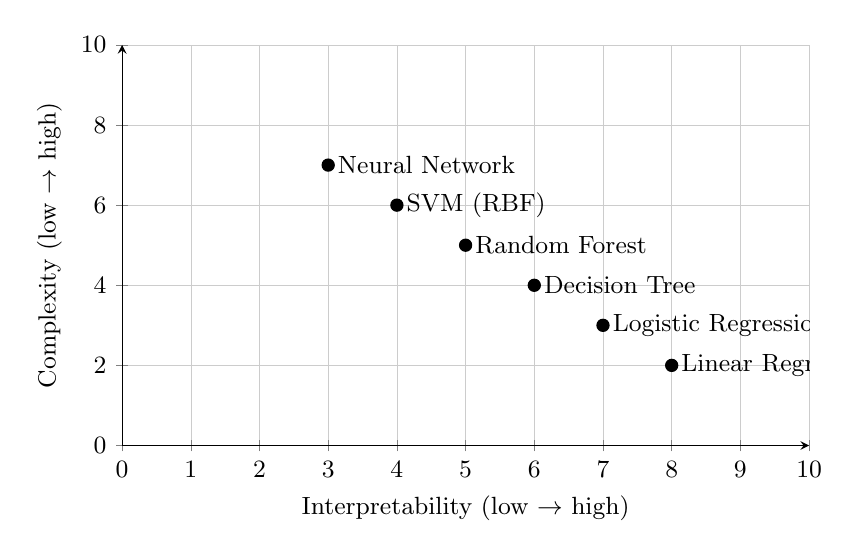
\begin{tikzpicture}
\begin{axis}[
    width=0.85\linewidth,
    height=0.55\linewidth,
    xlabel={Interpretability (low $\rightarrow$ high)},
    ylabel={Complexity (low $\rightarrow$ high)},
    xmin=0, xmax=10,
    ymin=0, ymax=10,
    grid=both,
    major grid style={line width=0.2pt, draw=gray!40},
    minor grid style={line width=0.1pt, draw=gray!20},
    tick label style={font=\small},
    label style={font=\small},
    axis lines=left,
]

\addplot[
    only marks,
    mark=*,
    mark size=2.2pt,
    color=black
] coordinates {
    (8,2) [Linear Regression]
    (7,3) [Logistic Regression]
    (6,4) [Decision Tree]
    (5,5) [Random Forest]
    (4,6) [SVM (RBF)]
    (3,7) [Neural Network]
};

\node[anchor=west, font=\small] at (axis cs:8,2) {Linear Regression};
\node[anchor=west, font=\small] at (axis cs:7,3) {Logistic Regression};
\node[anchor=west, font=\small] at (axis cs:6,4) {Decision Tree};
\node[anchor=west, font=\small] at (axis cs:5,5) {Random Forest};
\node[anchor=west, font=\small] at (axis cs:4,6) {SVM (RBF)};
\node[anchor=west, font=\small] at (axis cs:3,7) {Neural Network};

\end{axis}
\end{tikzpicture}
\caption{Interpretability vs. complexity of common methods.}
\end{figure}


The second \textbf{tradeoff} is between \textbf{underfitting} vs \textbf{overfitting}. 
Your model should be complex enough to capture the underlying patterns in the data (avoiding underfitting), but not so complex that it captures noise or random fluctuations (avoiding overfitting). Techniques such as cross-validation, regularization, and early stopping can help manage this tradeoff.


\begin{mytheorem}[Assessing the performance of supervised learning models]
To evaluate the performance of supervised learning models, we can use various metrics depending on whether the task is regression or classification.
For regression tasks, common metrics include: cost/loss functions, Mean Squared Error (MSE) \eqref{eq:mse}, Root Mean Squared Error (RMSE), Mean Absolute Error (MAE), and R-squared (\(R^2\)).
For classification tasks, common metrics include: accuracy, precision, recall, F1-score, and Area Under the Receiver Operating Characteristic Curve (AUC-ROC curve).
%

If data are correlated, we can include some correlation matrix $\sigma$ in the cost function, e.g. for MSE we would have
\begin{align}
    J(W, b) = \frac{1}{n} \sum_{i=1}^{n} \left( y_i - \hat{y}(x_i) \right)^T \sigma^{-1} \left( y_i - \hat{y}(x_i) \right)
\end{align}
where the covariance matrix $\sigma$ encodes the correlations between different data points and is typically estimated from the training data.

Yet another method for linear regression if the negative log-likelihood. Assuming the errors are normally distributed with mean zero and variance \(\sigma^2\), the negative log-likelihood can be expressed as:
\begin{align}
    J = \frac{1}{2\sigma^2} \sum_{i=1}^{n} \left( y_i - \hat{y}(x_i) \right)^2 + \frac{n}{2} \log(2\pi\sigma^2)
\end{align}
Minimizing this negative log-likelihood is equivalent to minimizing the MSE, but it provides a probabilistic interpretation of the model.

Another method for binary classification is cross-entropy loss. Given true labels \(y_i\) (0 or 1) and predicted probabilities \(\hat{y}(x_i)\), the cross-entropy loss is defined as:
\begin{align}
    J = -\frac{1}{n} \sum_{i=1}^{n} \left[ y_i \log(\hat{y}(x_i)) + (1 - y_i) \log(1 - \hat{y}(x_i)) \right]
\end{align}
This loss function penalizes incorrect predictions more heavily, especially when the predicted probability is far from the true label.
%
\end{mytheorem}



\begin{mytheorem}[Issues of supervised learning]
There are several problems we sould rather avoid and side aim to achieve.
\begin{itemize}
    \item The model should NOT learn the noise in the training data (overfitting). 
    \item The model should generalize well to unseen data (avoid underfitting).
\end{itemize}
To address these issues, we typically split the dataset into training, validation, and test sets. The training set is used to train the model, the validation set is used to tune hyperparameters and assess model performance during training, and the test set is used to evaluate the final model's performance on unseen data.

The best way to assess the optimal capacity is to stop when capacity is such that the \textbf{bias} and the \textbf{variance} cross each other.
Indeed, overfitting is associated with high variance and low bias, while underfitting is associated with high bias and low variance. The goal is to find a balance between bias and variance that minimizes the overall prediction error (cf. plots).
%

To penalize overfitting we can add weights to the cost function that penalize large coefficients, which would make the model very sensible to small changes in the input.
For example in linear regression we can add a regularization term to the cost function:
\begin{align}
    J(W, b) = \frac{1}{n} \sum_{i=1}^{n} \left\| y_i - \hat{y}(x_i) \right\|^2 + \lambda \|W\|^2
\end{align}
Such a term is called L2 regularization (or Ridge regularization) and helps prevent overfitting by discouraging large weights $W$ in the model. The hyperparameter \(\lambda\) controls the strength of the regularization. A larger \(\lambda\) increases the penalty for large weights, leading to a simpler model, but a huge \(\lambda\) will lead to underfitting!
\end{mytheorem}



%----------------------------------------------------
\part{Numerical Methods \& Optimization}

% !TeX root = ../comp_methods_main.tex
%==========================================================
%=========================================================
\chapter{Numerical Methods for PDEs}
%=========================================================
%=========================================================





% !TeX root = ../comp_methods_main.tex
%==========================================================
%=========================================================
\chapter{Numerical Linear Algebra}
%=========================================================
%=========================================================


%-----------------------------------------------------------------------
%======================================================================
\section{Matrix decompositions}
%========================================================================
%--------------------------------------------------------


% !TeX root = ../comp_methods_main.tex
%==========================================================
%=========================================================
\chapter{Optimization}
%=========================================================
%=========================================================


%-----------------------------------------------------------------------
%======================================================================
\section{Convex Optimization}
%========================================================================
%--------------------------------------------------------







%----------------------------------------------------
\part{Computational \& Statisical Softwares}

%\input{body/statistical_software.tex}

% !TeX root = ../comp_methods_main.tex
%==========================================================
%=========================================================
\chapter{Mathematica}
%=========================================================
%=========================================================


%-----------------------------------------------------------------------
%======================================================================
\section{Symbolic computation}
%========================================================================
%--------------------------------------------------------




\end{document}
